% CONVERTING TO PNG:
% http://www.graphicsmagick.org
% gm convert -density 300 -antialias -transparent white overview.pdf overview.png


\documentclass[tikz, margin=2mm]{standalone}
\usetikzlibrary{arrows.meta,arrows}


\usepackage{bold-extra}
\usepackage{xcolor}
\definecolor{darkgreen}{RGB}{19,138,7}
\definecolor{darkblue}{RGB}{7,19,138}

\begin{document}

\begin{tikzpicture}
    
\filldraw[color=black!90, fill=black!30, very thick]
    (0,0) rectangle (5,3)
    node[pos=.5] (binary) {\textcolor{darkgreen}{\texttt{\textbf{\Large Binary}}}};

\node[draw=none,text width=4.5cm] at (2.5,-1.5)  {
  \large
  \begin{tabular}{ll}
    Format: & ELF / Mach-O \\
    Arch:   & x86-64\\
    Convention: & System V AMD64 ABI\\
    Assumptions: & No concurrency
  \end{tabular}
  } ;


\draw[-{Stealth[length=6mm, width=4mm]}] (5,1.5) -- (7.5,1.5);

\filldraw[color=blue!60, fill=blue!5, very thick,rounded corners]
    (7.5,0.5) rectangle (12.5,2.5)
    node[pos=.5]  (foxdec) {\textcolor{darkblue}{\texttt{\textbf{\Large FoxDec}}}} ;

\draw[-{Stealth[length=6mm, width=4mm]}] (12.5,1.5) -- (15,1.5);

\filldraw[color=black!90, fill=black!30, very thick]
    (15,0) rectangle (20,3)
    node[pos=.5] (report) {\textcolor{darkgreen}{\texttt{\textbf{\Large Report}}}};

\draw[-{Stealth[length=6mm, width=4mm]}] (20,1.5) -- (22.5,1.5);

\filldraw[color=blue!60, fill=blue!5, very thick]
    (22.5,4) rectangle (28.5,3)
    node[pos=.5] (report) {
         \begin{tabular}{c}
            \textcolor{darkblue}{\texttt{\textbf{\Large <<interface>>}}}\\
            \textcolor{darkblue}{\texttt{\textbf{\Large VerificationReport}}}
          \end{tabular}
         };
\filldraw[color=blue!60, fill=blue!5, very thick]
    (22.5,3) rectangle (28.5,-1)
    node[pos=.5] (report) {
         \begin{tabular}{l}
            \textcolor{darkblue}{\texttt{\textbf{get\_instruction}}}\\
            \textcolor{darkblue}{\texttt{\textbf{\hspace{3ex} :: Address -> Instr}}}\\
            \textcolor{darkblue}{\texttt{\textbf{get\_invariant}}}\\
            \textcolor{darkblue}{\texttt{\textbf{\hspace{3ex} :: Address -> Invariant}}}\\
            \textcolor{darkblue}{\texttt{\textbf{get\_indirections}}}\\
            \textcolor{darkblue}{\texttt{\textbf{\hspace{3ex} :: Address -> \{Address\}}}}\\
            \textcolor{darkblue}{\texttt{\textbf{\ldots}}}\\
            \textcolor{darkblue}{\texttt{\textbf{\ldots}}}
          \end{tabular}
         };


\draw[-{Stealth[length=6mm, width=4mm]}] (16,-1) -- (15,-2.5);
\node[inner sep=0pt] (isabelle) at (14,-4) {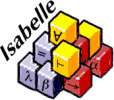
\includegraphics[width=3cm]{isabelle_logo.jpg}};


\draw[-{Stealth[length=6mm, width=4mm]}] (17.5,-1) -- (17.5,-2.5);
\filldraw[color=blue!60, fill=blue!5, very thick,rounded corners]
    (16.5,-6) rectangle (18.5,-2.75)
    node[pos=.5,rotate=60]  {\textcolor{darkblue}{\texttt{\textbf{\Large Disassembly}}}} ;


\draw[-{Stealth[length=6mm, width=4mm]},dashed] (19,-1) -- (20,-2.5);
\filldraw[color=blue!60, fill=blue!5, very thick,rounded corners,dashed]
    (19.5,-6) rectangle (22,-2.75)
    node[pos=.5,rotate=60]{
       \begin{tabular}{c}
         \textcolor{darkblue}{\texttt{\textbf{\Large Variable}}}\\
         \textcolor{darkblue}{\texttt{\textbf{\Large Analysis}}}
       \end{tabular}};

\end{tikzpicture}
\end{document}
